\section{Results and Discussion}\label{sec:result}
{\color{red}{show every step of results and analysis, show Figure~\ref{fig:result}, limitation, more results Figure~\ref{fig:more}}}

The step of shape optimization in our paper can be best demonstrated on the model~\ref{fig:result}, through initialization, we can have a rough concept of the final model, and by user interaction, we can finally generate a pleasing model from a given structural layout.

We show a number of 3D models generated by our system~\ref{fig:more}, and most of the cases can have an ideal result after initialization because of the common shape. However, the initialization will not generate a pleasing result on some complicated cases Figure~\ref{fig:limitation}, and leads to the difficult interaction to get the final model. 


\begin{figure}
	\centering
	\includegraphics[width=0.9\textwidth]{images/result.jpg}
	\caption{}
	\label{fig:result}
\end{figure}

\begin{figure}
	\centering
	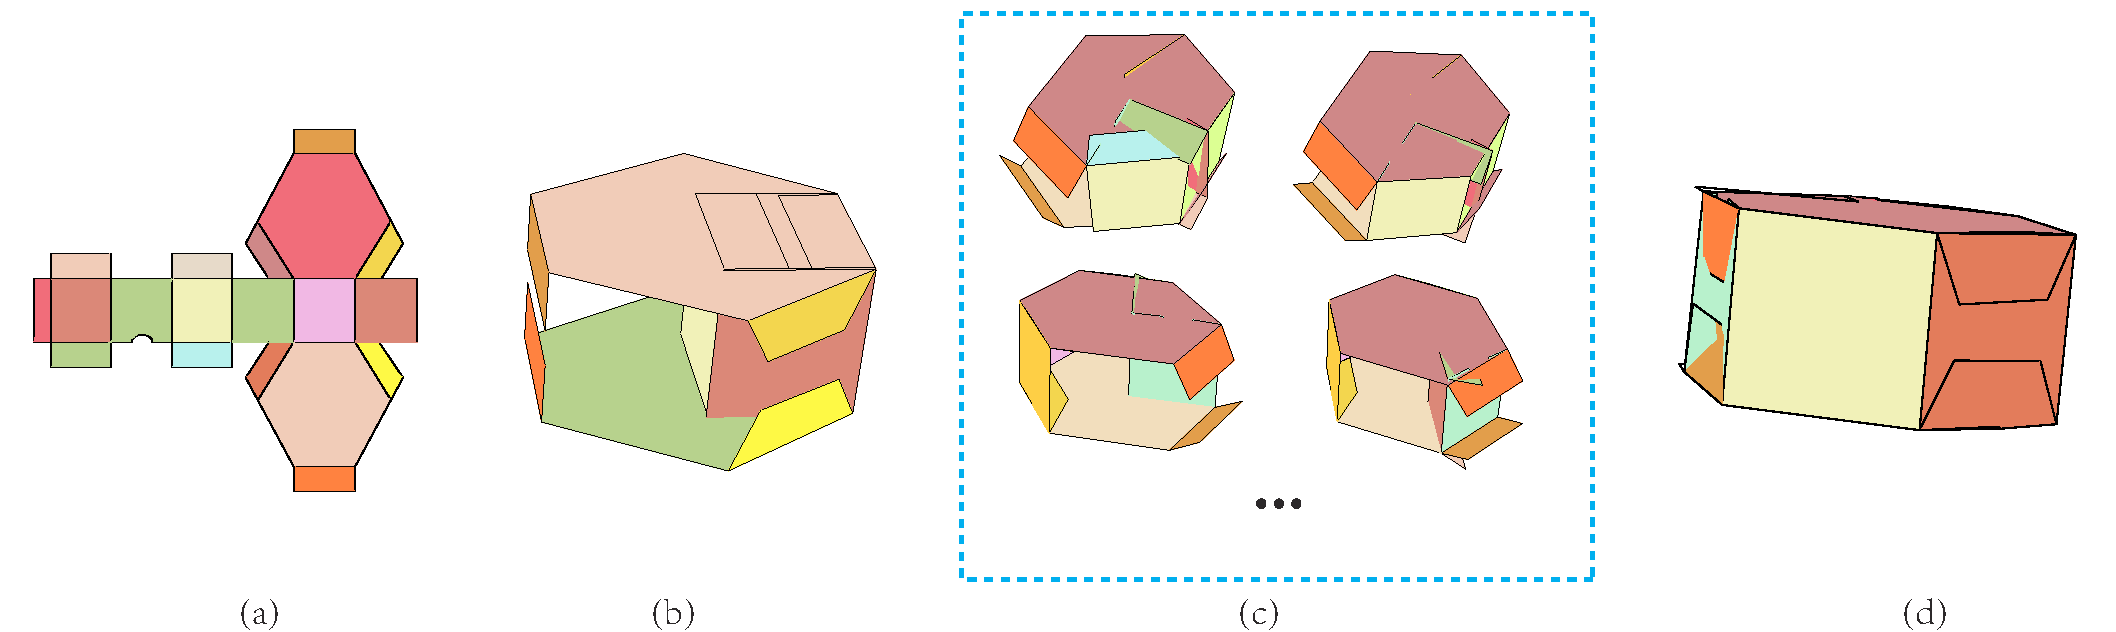
\includegraphics[width=0.9\textwidth]{images/limitation.jpg}
	\caption{Given a layout as (a), our system can generate an initialized result as (b). Although we know it's a hexagonal box, it's difficult to select the vertex we want as they are relocated together.}
	\label{fig:limitation}
\end{figure}

\begin{figure}
	\centering
	\includegraphics[width=0.9\textwidth]{images/more.jpg}
	\caption{More results, the first column is the flat mesh of a carton generated by given layout, the second column is the initialization result, and the last column is the result after interaction.}
	\label{fig:more}
\end{figure}